\documentclass[titlepage=firstcover, captions=tableheading]{scrartcl}
\usepackage{microtype}
\usepackage{amsmath}
\usepackage{polyglossia}
\usepackage{graphicx}
\usepackage{booktabs}
\usepackage{siunitx}
\usepackage{hyperref}
\usepackage{caption}
\usepackage{float}
\setdefaultlanguage{german}
\title{206 Die Wärmepumpe}
\author{
Connor Magnus Böckmann \\ email: \href{mailto:connormagnus.boeckmann@tu-dortmund.de}{connormagnus.boeckmann@tu-dortmund.de}
\and Tim Theissel \\ email: \href{mailto:tim.theissel@tu-dortmund.de}{tim.theissel@tu-dortmund.de}  
}
\begin{document}
\maketitle
\newpage
\tableofcontents
\newpage
\section{Zielsetzung}
Der Versuch V206 "Die Wärmepumpe" dient zur Untersuchung des Transports von Wärmeenergie entgegen des Wärmeflusses, 
wobei die reale Güteziffer der Wärmepumpe, der Massendurchsatz und der Wirkungsgrad des Kompressors bestimmt werden. 
Diese Kenngrößen sind ausschlaggebend für die Qualität der im Versuch verwendeten Wärmepumpe. 

\section{Theoretische Grundlagen} 

Eine Wärmepumpe dient dem Transport von Wärme von einem kälteren zu einem wärmeren Reservoir. 
Wärme fließt aber nach dem zweiten Hauptsatz der Thermodynamik immer von einem wärmeren zu einem kälteren Reservoir, 
weshalb bei der Wärmepumpe mechanische Arbeit verrichtet werden muss, um diesen Ablauf umzukehren. 
\subsection{Güteziffer}
Unter idealisierenden Bedingungen soll das Verhältnis aus transportierter Wärmemenge und der mechanischen Arbeit A, 
welche zum Wärmetransport aufgebracht werden muss, ausgerechnet werden. 
Eben dieses Verhältnis wird Güteziffer v einer Wärmepumpe genannt. 
Dem ersten Hauptsatz der Thermodynamik folgend, geht hervor dass die Wärmemenge Q\textsubscript{2},
welche aus dem kälteren Reservoir abgeführt wurde,
und die aufgebrachte mechanische Arbeit A in Summe der an das wärmere Reservoir abgegebenen Wärmemenge Q\textsubscript{1} entspricht.

\begin{equation}\label{1}
    Q_1= Q_2+A 
\end{equation}

\noindent Das oberhalb beschriebene Verhältnis aus Wärmemenge Q\textsubscript{1} und mechanischer Arbeit A, also Güteziffer v, ergibt sich zu: 

\begin{displaymath}
    v = \frac{Q_1}{A}
\end{displaymath}

\noindent Eine weitere entscheidende Beziehung zwischen zwei Temperaturen T\textsubscript{1} und T\textsubscript{2} 
und den Wärmemengen Q\textsubscript{1} und Q\textsubscript{2} entstammt dem zweiten Hauptsatz der Thermodynamik.
Wenn sich die Temperaturen der beiden Reservoirs T\textsubscript{1} und T\textsubscript{2} während des Wärmetransports nicht ändern,
verschwinden die summierten reduzierten Wärmemengen.  

\begin{equation}\label{3}
    \frac{Q_1}{T_1} - \frac{Q_2}{T_2} = 0
\end{equation}

\noindent Damit die Gleichung \ref{3} allerdings funktioniert muss eine idealisierende Annahme getroffen werden. 
Damit die Gleichung gilt muss die Wärmeübertragung nämlich vollständig reversibel, also umgekehrt werden können. 
Dies ist in der Realität aber nicht möglich. Für realitätsgenaue Berechnungen gilt also eigentlich: 

\begin{displaymath}
    \frac{Q_1}{T_1} - \frac{Q_2}{T_2} > 0
\end{displaymath} 

Aus \ref{1} und \ref{3} folgt dann 

\begin{displaymath}
    Q_1 = A + \frac{T_2}{T_1} \cdot Q_1
\end{displaymath}

, für die Güteziffer einer idealisierten Wärmepumpe 

\begin{equation}
    \nu_{id} = \frac{Q_1}{A} = \frac{T_1}{T_1 - T_2}
\end{equation}

und für die reale Wärmepumpe dementsprechend  

\begin{displaymath}
    \nu_{real} < \frac{T_1}{T_1 - T_2} .
\end{displaymath}

\noindent Aus (4) folgt, dass die Wärmepumpe umso günstiger funktioniert, wenn die Temperaturdifferenz zwischen T1 und T2 gering ist, 
also die beiden Reservoirs ähnlich warm sind.
Verwendet werden derartige Wärmepumpen zur kostengünstigen Beheizung, 
da die Wärmemenge Q2 einem kostenlos zur Verfügung stehenden Reservoir wie etwa der Luft oder dem Grundwasser entnommen wird. 
Daher muss der Betreiber nur Kosten für die mechanische Arbeit tragen, um Q2 = Q1 - A aus dem Reservoir zu pumpen.
Die erhaltene Wärme ist hierbei potenziell höher als die aufgebrachte mechanische Arbeit

\begin{displaymath}
    Q_{1_{rev}} = A \frac{T_1}{T_1 - T_2}.
\end{displaymath} 


\noindent Die reale Güteziffer lässt sich durch den Differentialquotienten $\Delta$T1/$\Delta$t für das Zeitintervall $\Delta$ t berechnen.
Des Weiteren wird die Wärmemenge $\Delta$Q1/$\Delta$t benötigt nach 
\begin{displaymath}
    \frac{\Delta Q_1}{\Delta t} = (m_1c_w + m_kc_k)\frac{\Delta T_1}{\Delta t}
\end{displaymath}
wobei $m_1c_w$ die Wärmekapazität des Wassers und m\textsubscript{k}c\textsubscript{k} die Wärmekapazität der Apparatur darstellt.
 N ist die von einem Wattmeter angezeigte und gemittelte Leistung des Kompressors. Die reale Güteziffer ist damit 
 
 \begin{equation} \label{eqn:gute}
    \nu = \frac{\Delta Q_1} {\Delta t N}.
 \end{equation}

 \subsection{Massendurchsatz}

 Die Vorschrift 
\begin{displaymath}
    \frac{\Delta Q_2}{\Delta t}=(m_2c_w + m_kc_k)\frac{\Delta T_2}{\Delta t}
\end{displaymath}

 stellt die pro Zeitintervall entnommene Wärmemenge dar.
 Außerdem gilt 
 \begin{displaymath}
     \frac{\Delta Q_2}{\Delta t} = L\frac{\Delta m}{\Delta t}
 \end{displaymath} 
 L ist dabei die Verdampfungswärme des Transportmediums. 
 Daraus ergibt sich
\begin{equation} \label{massendurchsatz}
    \frac{\Delta m}{\Delta t} = (m_2c_w + m_kc_k)\frac{\Delta T_2}{\Delta t L}
    = \frac{\Delta Q_2}{\Delta t} \cdot \frac{1}{L}.
\end{equation}

\subsection{Kompressorleistung N\textsubscript{mech}}

Für die Komprimierung des Gasvolumens von V\textsubscript{a} auf V\textsubscript{b} benötigte Arbeit A\textsubscript{m} gilt 

\begin{displaymath}
    A_m = -\int_{V_a}^{V_b} p \: dV
\end{displaymath} 

\noindent Mit $ N_{mech} = \frac{\delta A_m}{\delta t} $ und der Poissonschen Gleichung ergibt sich
\begin{equation} \label{kompressorleistung}
    N_{mech} =\frac{\Delta A_m}{\Delta t} 
    = \frac{1}{\kappa -1} \left(p_b\sqrt[\kappa]{\frac{p_a}{p_b}}-p_a\right) \frac{\Delta V_a}{\Delta t}
    = \frac{1}{\kappa -1} \left(p_b\sqrt[\kappa]{\frac{p_a}{p_b}}-p_a\right) \frac{1}{\rho} \frac{\Delta m}{\Delta t}
\end{equation}

\noindent mit \rho \: als Dichte des Mediums im gasförmigen Zustand und \kappa , dem Verhältnis der Molwärmen, c\textsubscript{p} und c\textsubscript{v}.

\subsection{Gauß-Fehler}

Der Gauß- Fehler wird in verschiedenen Abschnitten berechnet, jedoch immer nach der folgenden Formel der Gauß'schen Fehlerfortpflanzung:

\begin{equation} \label{4}
    \Delta f = \sqrt{\left(\frac{(\partial f)²}{(\partial x)²}\right) (\Delta x)² +
                     \left(\frac{(\partial f)²}{(\partial y)²}\right) (\Delta y)² + ... +
                     \left(\frac{(\partial f)²}{(\partial z)²}\right) (\Delta z)²
    }
\end{equation}

\section{Aufbau und Funktionsweise einer Wärmepumpe}

Im Folgenden wird die prinzipielle Funktionsweise einer Wärmepumpe, wie sie zur Durchführung des Versuchs verwendet wird, genauer beschrieben. 

\noindent Die Wärmepumpe funktioniert auf dem Prinzip der Phasenumwandlung. 
Dazu wird ein reales Gas als Medium zum Transport der Wärme benutzt. 
Dieses nimmt während des Verdampfens Energie auf und gibt diese bei der Kondensation wieder ab. 
Daher sollte ein Medium mit möglichst großer Kondensationswärme gewählt werden.  
\begin{figure}[H]
    \centering
    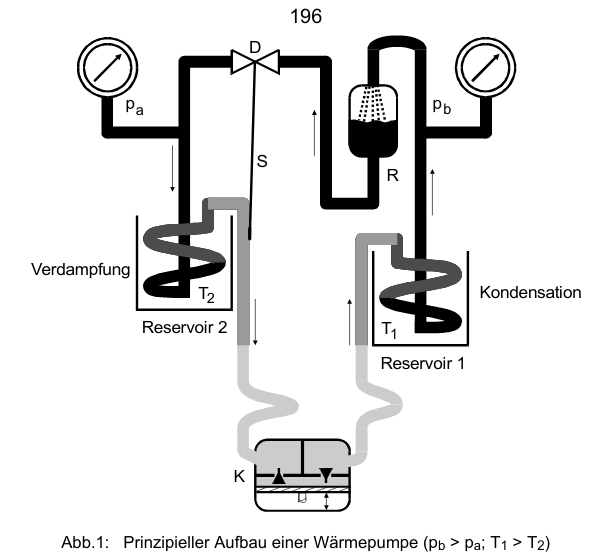
\includegraphics[height=8cm]{Abb1}
    \captionbelow{TU Dortmund.Versuchsanleitung zum Experiment V206 - Die Wärmepumpe Seite 196.}
\end{figure}

\noindent Der schematische Aufbau einer Wärmepumpe wird in Abb. 1 dargestellt. 
Sie besteht aus einem geschlossenen Mediumkreislauf, welcher durch den Kompressor K erzeugt wird und durch die beiden Reservoirs 1 und 2 verläuft. 
Außerdem durchströmt das Medium das Drosselventil D, an welchem sich eine Druckdifferenz p\textsubscript{b}-p\textsubscript{a} einstellt. 
Das Medium soll dabei bei der Temperatur T1 und dem Druck p\textsubscript{b} flüssig und bei dem Druck p\textsubscript{a} und der Temperatur T2 gasförmig sein. 
Das flüssige Medium verdampft beim Durchfließen von Reservoir 2, wodurch es dem Reservoir die Verdampfungswärme L entzieht. 
Das Reservoir 2 stellt also die kalte Seite da und gibt somit Wärme ab. 
Das Medium wird daraufhin vom Kompressor so adiabatisch komprimiert, dass es sich erwärmt, sich der Druck erhöht und in Reservoir 1 kondensiert 
und die Kondensationswärme L abgibt.\\

\noindent Für die reibungslose Funktion werden noch ein Reiniger, welcher die Flüssigkeit gasblasenfrei macht, 
und eine Steuervorrichtung für das Drosselventil, welche dafür sorgt, dass nur Gas in den Kompressor gelangt und keine Flüssigkeitsreste, benötigt. 
Diese Bauteile haben mit der theoretischen Arbeitsweise der Apparatur nichts zu tun, werden aber für eine gute Funktion benötigt. 

\pagebreak

\section{Durchführung}
Die Versuchsapparatur sieht schematisch folgendermaßen aus:
\begin{figure}[H]
    \centering
    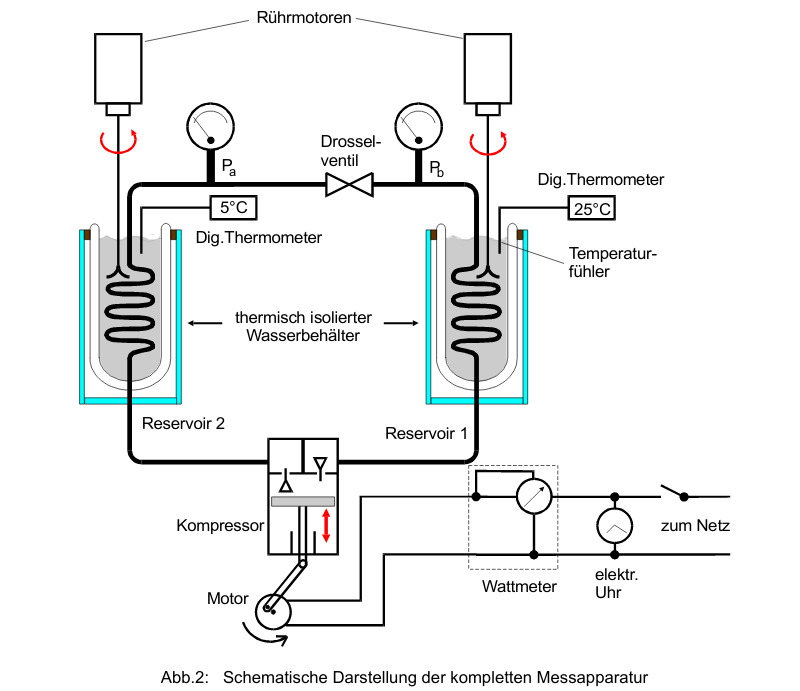
\includegraphics[height=9cm]{Abb2.png}
    \captionbelow{TU Dortmund.Versuchsanleitung zum Experiment V206 - Die Wärmepumpe Seite 197.}
\end{figure}
\noindent Vor Beginn sind die Anfangsdrücke und Temperaturen aufzunehmen. 
Daraufhin werden die beiden Reservoirs mit genau abgemessenen 4l Wasser befüllt und die Wärmekapazität m\textsubscript{k}g\textsubscript{k}=750$\frac{J}{K}$ notiert. 
Nun wird der Kompressor eingeschaltet und in Abständen von einer Minute die Temperaturen T\textsubscript{1} und  T\textsubscript{2}, 
die Drücke p\textsubscript{a} und p\textsubscript{b}, 
die Zeit und die Leistungsaufnahme des Kompressors von den Thermo- und Manometern beziehungsweise dem Wattmeter aufgenommen. 
Auf die abgelesenen Drücke muss jeweils immer noch 1 bar addiert werden. 
Die Messung wird abgebrochen, wenn die Temperatur T\textsubscript{1} einen Wert von 50°C übersteigt. 

\section{Messwerte/Auswertung}

Zu Beginn der Auswertung werden in diesem Abschnitt alle gemessenen Werte in einer Tabelle dargestellt. Außerdem wurden hier die Temperaturen von °C in °K umgerechnet,
da diese im weiteren Verlauf der Rechnung auch in dieser Einheit verwendet werden.
Die Auswertung beschäftigt sich dann mit der Berechnung aller wichtigen Kenngrößen aus den gemessenen Größen unter Betrachtung des Gauß-Fehlers, 
der durch die Messungenauigkeiten bei der Durchführung des Versuchs entsteht und sich durch weitere Rechnungen fortpflanzt. 
\noindent
\begin{minipage}{\linewidth}
\begin{center}
    \captionof{table}{Gemessene Werte}
        \begin{tabular}{lllllllr}  
            \toprule
            Zeit t (s)    & T\textsubscript{1} (°C) & p\textsubscript{b} (bar) & T\textsubscript{2} (°C) & p\textsubscript{a} (bar) & N (W) & T\textsubscript{1} (K) 
            & T\textsubscript{2} (K) \\
            \midrule
            0   	&   21.7 & 4.0 &    21.7 &  4.1 &   120   & 294.85 & 294.85 \\
            60  	&   23.0 & 5.0 &	21.7 &  3.2	&   120   & 296.15 & 294.85  \\
            120 	&   24.3 & 5.5 &	21.6 &	3.4	&   120   & 297.45 & 294.75  \\
            180 	&   25.3 & 6.0 &	21.5 &	3.5	&   120   & 298.45 &  294.65 \\
            240 	&   26.4 & 6.0 & 	20.8 &	3.5	&   120   & 299.55 & 293.95  \\
            300 	&   27.5 & 6.0 & 	20.1 &	3.4 &	120   & 300.65 & 293.25  \\
            360 	&   28.8 & 6.5 & 	19.2 &	3.3 &	120   & 301.95 & 292.35  \\
            420 	&   29.7 & 6.5 & 	18.5 &	3.2 &	120   & 302.85 & 291.65  \\
            480 	&   30.9 & 7.0 & 	17.7 &	3.2 &	120   & 304.05 & 290.85  \\
            540 	&   31.9 & 7.0 & 	16.9 &	3.0 &	120   & 305.05 & 290.05  \\
            600 	&   32.9 & 7.0 & 	16.2 &	3.0 &	120   & 306.05 & 289.35    \\
            660 	&   33.9 & 7.5 & 	15.5 &	2.9 &	120   & 307.05 & 288.65  \\
            720 	&   34.8 & 7.5 &	14.9 &	2.8 &	120   & 307.95 & 288.05  \\
            780 	&   35.7 & 8.0 & 	14.2 &	2.8 &	120   & 308.85 & 287.35 \\
            840 	&   36.7 & 8.0 &	13.6 &	2.7 &	120   & 309.85 & 286.75  \\
            900 	&   37.6 & 8.0 &	13.0 &	2.6 &	120   & 310.75 & 286.15  \\
            960 	&   38.4 & 8.5 & 	12.4 &	2.6 &	120   & 311.55 & 285.55  \\
            1020	&   39.2 & 8.5 & 	11.7 &	2.6 &	120   & 312.35 & 284.85  \\
            1080	&   40.0 & 9.0 & 	11.3 &	2.5 &	120   & 313.15 & 284.45  \\
            1140	&   40.7 & 9.0 & 	10.9 &	2.5 &	120   & 313.85 & 284.05  \\
            1200	&   41.4 & 9.0 & 	10.4 &	2.4 &	120   & 314.55 & 283.55  \\
            1260	&   42.2 & 9.0 & 	 9.9 &  2.4 &	120   & 315.35 & 283.05  \\
            1320	&   42.9 & 9.5 & 	 9.5 &	2.4 &   120   & 316.05 & 282.65  \\
            1380	&   43.6 & 9.5 & 	 9.1 &	2.4	&   120   & 316.75 & 282.25  \\
            1440	&   44.3 & 10.0 &	 8.7 &	2.4 &	120   & 317.45 & 281.85 \\
            1500	&   44.9 & 10.0 &	 8.3 &	2.4 &	120   & 318.05 & 281.45  \\
            1560	&   45.5 & 10.0 &	 8.0 &	2.3 &	120   & 318.05 & 281.15  \\
            1620	&   46.1 & 10.0 &	 7.7 &	2.2 &	122   & 319.25 & 280.85  \\
            1680	&   46.7 & 10.5 &	 7.4 &	2.2 &	122   & 319.85 & 280.55  \\
            1740	&   47.3 & 10.5 &	 7.1 &	2.2 &	122   & 320.45 & 280.25  \\
            1800	&   47.8 & 10.75 &	 6.8 &	2.2 &	122   & 320.95 & 279.95 \\
            1860	&   48.4 & 11.0 &	 5.6 &	2.2 &	122   & 321.55 & 278.75  \\
            1920	&   48.9 & 11.0 &	 4.3 &	2.2 &	122   & 322.05 & 277.45  \\
            1980	&   49.4 & 11.0 &	 3.4 &	2.2 &	122   & 322.55 & 276.55  \\
            2040	&   49.9 & 11.0 &	 3.0 &	2.2 &	122   & 323.05 & 276.15  \\
            2100	&   50.3 & 11.0 &	 2.9 &	2.2	&   122   & 323.45 & 276.05  \\
            \bottomrule
        \end{tabular}
    \end{center}
    
\end{minipage}  
\subsection{Aufgabe 5a) und 5b)}   

In dieser Aufgabe sollen die Temperaturverläufe dargestellt werden und dann mit Hilfe einer nicht linearen Ausgleichsrechnung approximiert werden. 
Dafür werden die Messwerte für die verschiedenen Temperaturen in Kelvin auf der x-Achse und die jewilige Zeit auf der y-Achse dargestellt. 
Außerdem werden die Graphen der Ausgleichsrechnungen noch in diesem Diagramm eingezeichnet.

\begin{center}
    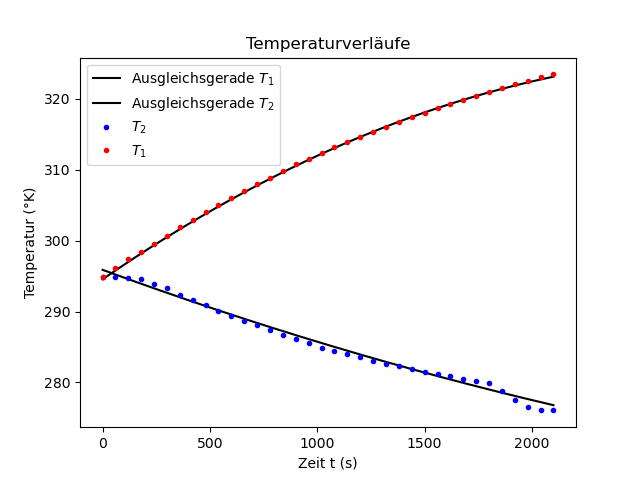
\includegraphics[height=8cm]{plot2.png}
\end{center}
Bestimmung der Parameter der Näherungsfunktionen: 
Eine nicht-lineare Ausgleichsrechnung in mycurvefit.com mittels der Funktion $At^2+Bt+C$ ergibt die folgenden Parameter: 
Für T\textsubscript{1}:

\begin{center}
    
\begin{tabular}{
    l
    r
    @{${}\pm{}$}
    r
}
    \toprule
    {Parameter} & {T\textsubscript{1}(t)} & {Fehler} \\
    \midrule
    A & -$3.47 * 10^{-6}$ &  $0.227 *10^{-6}$ \\
    B & $2.09 * 10^{-2} $&  $0.0475 * 10^{-2} $ \\
    C & 294.54 &  0.1732 \\
    \bottomrule
\end{tabular}
\end{center}

Und für T\textsubscript{2}:(5)

\begin{center}
\begin{tabular}{
    l
    r
    @{${}\pm{}$}
    r
}
    \toprule
    {Parameter} & {T\textsubscript{2}(t)} & {Fehler} \\
    \midrule
    A & $9.563 * 10^{-6} $ &  $0.4694 * 10^{-6} $ \\
    B & $ -1.11 * 10^{-2} $&  $ 0.094 * 10^{-2} $ \\
    C & 295.88 &  0.3465 \\
    \bottomrule
\end{tabular}
\end{center}

\subsection{Aufgabe 5c)}
Bestimmung der Differentialquotienten: 
Nun werden aus ebendieser Funktion $At^2+Bt+C$ die Differentialquotienten $\frac{dT_1}{dt}$ und $\frac{dT_2}{dt}$  zu vier verschiedenen Zeiten berechnet. 
Als Temperaturen wurden die Temperaturen nach 300s, 600s, 900s und 1200s gewählt. 
Der Differentialquotient ergibt sich dabei aus der Ableitung der Näherungsfunktion: 

\begin{displaymath}
    \frac{dT}{dt}=2At+B
\end{displaymath}

\noindent Mit den Parametern aus 5b) ergeben sich folgende Differentialquotienten und Gauß-Fehler nach \eqref{4}

Für T\textsubscript{1}:
\begin{center}
    \begin{tabular}{
        l
        r
        r
        r
    }
        \toprule
        {Zeit t (s)} & {T\textsubscript{1}(K)} & {$\frac{dT_1}{dt} $} & {Gauß-Fehler} \\
        \midrule
        300 & 300.65 &  $1.88  * 10^{-2}$& $0.04941 * 10^{-2}$ \\
        600 & 306.05 &  $1.67  * 10^{-2}$& $0.05476 * 10^{-2}$\\
        900 & 310.75 &  $1.47  * 10^{-2}$& $0.06266 * 10^{-2}$\\
        1200 & 314.55 & $ 1.26 * 10^{-2}$ & $0.07228 * 10^{-2}$ \\
        \midrule
        Mittelwert & & $1.57*10^{-2}$ & \\
        Standardabweichung & & $2.6595*10^{-3}$ \\
        \bottomrule
    \end{tabular}
    \end{center}

    Und  für T\textsubscript{2}:
    \begin{center}
        \begin{tabular}{
            l
            r
            r
            r
        }
            \toprule
            {Zeit t (s)} & {T\textsubscript{2}(K)} & {$\frac{dT_2}{dt} $} & {Gauß-Fehler} \\
            \midrule
            300 & 293.25 & $-1.05*10^{-2}$ & $0.09813 * 10^{-2}$\\
            600 & 289.35 & $-9.952*10^{-3}$ & $1.096 * 10^{-3}$\\
            900 & 286.15 & $-9.3787*10^{-3}$ & $1.264 * 10^{-3}$\\
            1200 & 283.55 & $-8.8099*10^{-3}$ & $1.467 * 10^{-3}$\\
            \midrule
            Mittelwert & & $-9.6589*10^{-3}$ & \\
            Standardabweichung & & $7.3057*10^{-4}$ & \\
            \bottomrule
        \end{tabular}
        \end{center}
        \subsection{Aufgabe 5d)}
        Bestimmung der Güteziffer: Schließlich soll die empirische Güteziffer nach Gleichung \eqref{eqn:gute} und die ideale nach Gleichung \eqref{3} bestimmt werden.
        Auch hier ergibt sich der Guaß-Fehler nach \eqref{4} 
        Die Wärmekapazität der Apparatur beträgt 
        c\textsubscript{k}m\textsubscript{k}=750J/K. 
        Der c\textsubscript{w}m\textsubscript{w}-Wert ist die Wärmekapazität des Wassers beträgt 16736J/K und 
        errechnet sich durch Multiplikation der spezifischen Wärmekapazität des Wassers 
        von 4184J/kg*K mit der Masse von 4kg. 

        \begin{center}
            \begin{tabular}{lr@{${}\pm{}$}lrr}
                \toprule
                {Zeit t} & { Güteziffer (real)} & {Gauß Fehler} & {Güteziffer (ideal)} & {Abweichung in \%} \\
                \midrule
                300 & 2.739 & 0.07035  & 40.628 & 93.26 \\
                600 & 2.433 & 0.07797  & 18.326 & 86.72 \\
                900 & 2.142 & 0.08922 & 12.632 & 83.04 \\
                1200 & 1.836 & 0.10290 & 10.147 & 81.91\\
                \bottomrule
                
            \end{tabular}
        \end{center}
\subsection{Aufgabe 5e)}

Im Folgenden soll, für verschiedene Temperaturen, der Massendurchsatz des Transportgases berechnet werden.
Dafür wird die Verdampfungswärme benötigt, welche sich aus Messwerten un dem Umgebungsdruck bestimmen lässt.
Dazu wird die Dampfdruck-Kurve erstellt. 
Die Steigung dieser Ausgleichsgerade wird bestimmt und damit die Verdampfungswärme, die zur Berechnung des Massendurchsatzes von Nöten ist.

\begin{center}
    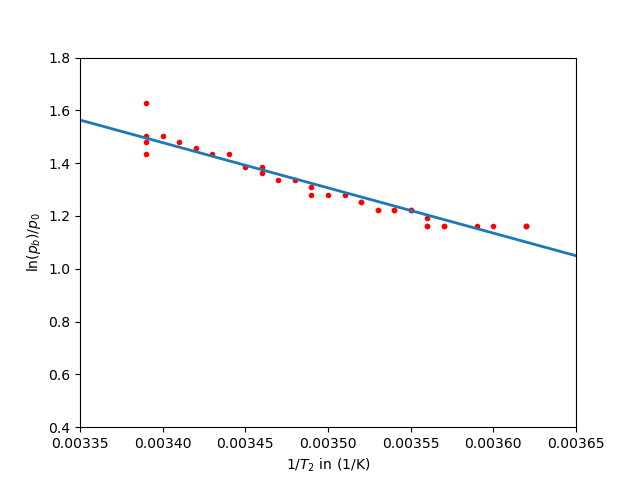
\includegraphics{massendurchsatz.png}
\end{center}
Dieses Diagramm stellt die Dampfdruck-Kurve dar.
Eine Lineare Regression mit der polyfit Funktion von numpy liefert die folgenden Werte für die Parameter der Ausgleichsfunktion: 
\begin{center}
    \begin{tabular}{r@{${}\pm{}$}rr@{${}\pm{}$}r}
        \toprule
        {Steigung} & {Fehler} & {Y-Achsenabschnitt} & {Fehler} \\
        \midrule
        -1713.315 & 88.019 & 7.303 & 0.308 \\
        \bottomrule
        
    \end{tabular}
\end{center}
Mit der Gleichung 
\begin{displaymath}
    L = -m*R ,
\end{displaymath}
wobei m die Steigung der Ausgleichsfunktion und R die universelle Gaskonstante ist,
lässt sich die Verdampfungswärme L bestimmen als 118,2639 J/g.
Für den Massendurchsatz dm/dt ergibt sich nach \eqref{massendurchsatz} mit dem Gauß-Fehler nach \eqref{4}: 
\begin{center}
    \begin{tabular}{lrrr}
        \toprule
        {Zeit t (s)} & {$dQ_2/dt$} & {$dm/dt$ (g/s)} & {Gauß-Fehler} \\
        \midrule
        300 & -183.603 & -1.5525 & 0.1654\\
        600 & -174.021 & -1.4715 & 0.1787\\
        900 & -163.996 & -1.3867 & 0.199\\
        1200& -153.962 & -1.3019 & 0.2269\\
        \bottomrule
        
    \end{tabular}
\end{center}

\subsection{Aufgabe 5f)}

Nun wird für die vier Temperaturen die Kompressorleistung berechnet, wennn er zwischen den Dürcken arbeitet,
die bei den verschiedenen Temperaturen herrschen.
Um dies zu erreichen wird Gleichung \eqref{kompressorleistung} mit den Parametern \rho = 5,51 kg/m³ als Dichte des Mediums,
\kappa = 1,14
dem Umgebungsdruck p\textsubscript{0} = 1 bar, der auf die gemessenen Drücke noch addiert werden muss. 
Der Gauß-Fehler berechnet sich mit \ref{4}.
\begin{center}
    \begin{tabular}{lr}
        \toprule
        {Zeit t (s)}  & {Leistung (W)} \\
        \midrule
        300 & $1.1967*10^{-4}$ \\
        600 & $1.6477*10^{-4}$ \\
        900 &  $2.0028*10^{-4}$\\
        1200& $2.1723*10^{-4}$ \\
        \bottomrule
        
    \end{tabular}
\end{center}
\section{Diskussion}
\subsection{Aufgabe 5g)}

Im Folgenden werden die errechneten Werte der realen Güteziffer mit denen der idealen Güteziffer verglichen.
Dabei werden auch mögliche Gründe für Abweichungen erörtert. 

\noindent Zu Beginn sind hier noch einmal wichtige Ergebnisse im Zusammenhang mit der Güteziffer dargestellt.
\begin{center}
    \begin{tabular}{lr@{${}\pm{}$}lrr}
        \toprule
        {Zeit t} & { Güteziffer (real)} & {Gauß Fehler} & {Güteziffer (ideal)} & {Abweichung in \%} \\
        \midrule
        300 & 2.739 & 0.07035  & 40.628 & 93.26 \\
        600 & 2.433 & 0.07797  & 18.326 & 86.72 \\
        900 & 2.142 & 0.08922 & 12.632 & 83.04 \\
        1200 & 1.836 & 0.10290 & 10.147 & 81.91\\
        \bottomrule
        
    \end{tabular}
\end{center}

\noindent Bei Betrachtung dieser Werte fällt schnell auf, dass der Unterschied zwischen realer und idealer Güteziffer enorm ist.
Die prozentuale Abweichung wird zwar mit der Zeit kleiner, ist aber auch am Ende bei über 80\% .
Um nun die Frage zu beantworten, warum diese Abweichungen so groß sind, lohnt es sich die reale und die ideale Wärmepumpe einmal zu vergleichen.
Die ideale Wärmepumpe ist perfekt isoliert. 
Das hat zur Folge, dass es keinen Wärmeverlust beim Transport des Gases durch die Apparatur gibt.
Nun ist aber die im Versuch verwendete Wärmepumpe eben keine Ideale. 
Das kann sie auch nicht sein, denn so eine perfekte Isolation wie sie die ideale Wärmepumpe fordert, ist praktisch nicht umsetzbar.
Einerseits sorgt dies für eine schlechtere Güteziffer, andererseits wird die Arbeit einer solchen realen Wärmepumpe irreversibel.
Mit einer idealen Wärmepumpe könnte der Prozess genauso gut umgekehrt werden.

\noindent Des Weiteren arbeitet auch der verwendete Kompressor nicht adiabatisch, 
d.h. das Komprimieren des Transportgases findet nicht ohne einen Wärmeaustausch mit der Umgebung statt.
Auch hier ist das System also nicht komplett thermisch abgeschlossen.
Daher wird hierdurch die Güteziffer der realen Wärmepumpe noch schlechter.

\noindent Außerdem müssen bei der Durchführung des Versuches verschiedene Messwerte wie beispielsweise die Temperatur genommen werden.
Dies ist eine Fehlerquelle, denn hier können Ungenauigkeiten durch Fehler der Messgeräte oder auch ungenaues Ablesen der Werte, die die Messgeräte liefern, entstehen.
Eine weitere Fehlerquelle wären auch eventuelle Rundungsfehler die durch automatisches Runden verwendeter Taschenrechner entstanden sein können.

\noindent Aufgrund der Tatsache, dass der Gauß-Fehler für die reale Güteziffer zwei Größenordnungen kleiner ist als der Wert der Güteziffer,
sind es vermutlich die Wärmeverluste, welche hauptsächlich für die hohe Abweichung verantwortlich sind. 

\section{Literatur}
TU Dortmund.Versuchsanleitung zum Experiment V206 - Die Wärmepumpe.\\
TU Dortmund.Daten und Hinweise zum Experiment V206 - Die Wärmepumpe.\\
PeP et al. Toolbox Workshop. Material zu SciPy. Aufruf vom 14.11.2020.\\
URL: https://toolbox.pep-dortmund.org/files/archive/2020/scientific-python.html

\end{document}
